%% abtex2-modelo-trabalho-academico.tex, v-1.9.2 laurocesar
%% Copyright 2012-2014 by abnTeX2 group at http://abntex2.googlecode.com/ 
%%
%% This work may be distributed and/or modified under the
%% conditions of the LaTeX Project Public License, either version 1.3
%% of this license or (at your option) any later version.
%% The latest version of this license is in
%%   http://www.latex-project.org/lppl.txt
%% and version 1.3 or later is part of all distributions of LaTeX
%% version 2005/12/01 or later.
%%
%% This work has the LPPL maintenance status `maintained'.
%% 
%% The Current Maintainer of this work is the abnTeX2 team, led
%% by Lauro César Araujo. Further information are available on 
%% http://abntex2.googlecode.com/
%%
%% This work consists of the files abntex2-modelo-trabalho-academico.tex,
%% abntex2-modelo-include-comandos and abntex2-modelo-references.bib
%%

% ------------------------------------------------------------------------
% ------------------------------------------------------------------------
% abnTeX2: Modelo de Trabalho Academico (tese de doutorado, dissertacao de
% mestrado e trabalhos monograficos em geral) em conformidade com 
% ABNT NBR 14724:2011: Informacao e documentacao - Trabalhos academicos -
% Apresentacao
% ------------------------------------------------------------------------
% ------------------------------------------------------------------------

\documentclass[
	% -- opções da classe memoir --
	12pt,				% tamanho da fonte
	openright,			% capítulos começam em pág ímpar (insere página vazia caso preciso)
	twoside,			% para impressão em verso e anverso. Oposto a oneside
	a4paper,			% tamanho do papel. 
	% -- opções da classe abntex2 --
	%chapter=TITLE,		% títulos de capítulos convertidos em letras maiúsculas
	%section=TITLE,		% títulos de seções convertidos em letras maiúsculas
	%subsection=TITLE,	% títulos de subseções convertidos em letras maiúsculas
	%subsubsection=TITLE,% títulos de subsubseções convertidos em letras maiúsculas
	% -- opções do pacote babel --
	english,			% idioma adicional para hifenização
	french,				% idioma adicional para hifenização
	spanish,			% idioma adicional para hifenização
	brazil				% o último idioma é o principal do documento
	]{abntex2}

% ---
% Pacotes básicos 
% ---
\usepackage{lmodern}			% Usa a fonte Latin Modern			
\usepackage[T1]{fontenc}		% Selecao de codigos de fonte.
\usepackage[utf8]{inputenc}		% Codificacao do documento (conversão automática dos acentos)
\usepackage{lastpage}			% Usado pela Ficha catalográfica
\usepackage{indentfirst}		% Indenta o primeiro parágrafo de cada seção.
\usepackage{color}				% Controle das cores
\usepackage{graphicx}			% Inclusão de gráficos
\usepackage{microtype} 			% para melhorias de justificação
% ---
		
% ---
% Pacotes adicionais, usados apenas no âmbito do Modelo Canônico do abnteX2
% ---
\usepackage{lipsum}				% para geração de dummy text
% ---

% ---
% Pacotes de citações
% ---
\usepackage[brazilian,hyperpageref]{backref}	 % Paginas com as citações na bibl
\usepackage[alf,abnt-emphasize=bf]{abntex2cite}	% Citações padrão ABNT

% --- 
% CONFIGURAÇÕES DE PACOTES
% --- 

% ---
% Configurações do pacote backref
% Usado sem a opção hyperpageref de backref
\renewcommand{\backrefpagesname}{Citado na(s) página(s):~}
% Texto padrão antes do número das páginas
\renewcommand{\backref}{}
% Define os textos da citação
\renewcommand*{\backrefalt}[4]{
	\ifcase #1 %
		Nenhuma citação no texto.%
	\or
		Citado na página #2.%
	\else
		Citado #1 vezes nas páginas #2.%
	\fi}%
% ---

% ---
% Informações de dados para CAPA e FOLHA DE ROSTO
% ---
\titulo{Classificação de discurso de ódio em memes com aprendizado multimodal para moderação de conteúdo nas redes sociais}
\autor{Ana Thayna Conceição França}
\local{SP - Brasil}
\data{2025}
\orientador{...}
\coorientador{...}
\instituicao{%
  Centro Universitário Senac - Santo Amaro
  \par
  Bacharelado em Ciência da Computação}
\tipotrabalho{Monografia}
% O preambulo deve conter o tipo do trabalho, o objetivo, 
% o nome da instituição e a área de concentração 
\preambulo{Monografia apresentada na disciplina Trabalho de Conclusão de Curso, como parte dos
requisitos para obtenção do título de Bacharel em Ciência da Computação.}
% ---



% ---
% Configurações de aparência do PDF final

% alterando o aspecto da cor azul
\definecolor{blue}{RGB}{41,5,195}

% informações do PDF
\makeatletter
\hypersetup{
     	%pagebackref=true,
		pdftitle={\@title}, 
		pdfauthor={\@author},
    	pdfsubject={\imprimirpreambulo},
	    pdfcreator={LaTeX with abnTeX2},
		pdfkeywords={abnt}{latex}{abntex}{abntex2}{trabalho acadêmico}, 
		colorlinks=true,       		% false: boxed links; true: colored links
    	linkcolor=blue,          	% color of internal links
    	citecolor=blue,        		% color of links to bibliography
    	filecolor=magenta,      		% color of file links
		urlcolor=blue,
		bookmarksdepth=4
}
\makeatother
% --- 

% --- 
% Espaçamentos entre linhas e parágrafos 
% --- 

% O tamanho do parágrafo é dado por:
\setlength{\parindent}{1.3cm}

% Controle do espaçamento entre um parágrafo e outro:
\setlength{\parskip}{0.2cm}  % tente também \onelineskip

% ---
% compila o indice
% ---
\makeindex
% ---

% ----
% Início do documento
% ----
\begin{document}

% Retira espaço extra obsoleto entre as frases.
\frenchspacing 

% ----------------------------------------------------------
% ELEMENTOS PRÉ-TEXTUAIS
% ----------------------------------------------------------
% \pretextual

% ---
% Capa
% ---
\imprimircapa
% ---

% ---
% Folha de rosto
% (o * indica que haverá a ficha bibliográfica)
% ---
%\imprimirfolhaderosto*
% ---

% ---
% Dedicatória
% ---
%\begin{dedicatoria}
   \vspace*{\fill}
   \centering
   \noindent
   \textit{ Este trabalho é dedicado às crianças adultas que,\\
   quando pequenas, sonharam em se tornar cientistas.} \vspace*{\fill}
\end{dedicatoria}
% ---

% ---
% Agradecimentos
% ---
%\begin{agradecimentos}
Os agradecimentos principais são direcionados à Gerald Weber, Miguel Frasson,
Leslie H. Watter, Bruno Parente Lima, Flávio de Vasconcellos Corrêa, Otavio Real
Salvador, Renato Machnievscz\footnote{Os nomes dos integrantes do primeiro
projeto abn\TeX\ foram extraídos de \url{http://codigolivre.org.br/projects/abntex/}} e todos aqueles que
contribuíram para que a produção de trabalhos acadêmicos conforme
as normas ABNT com \LaTeX\ fosse possível.

Agradecimentos especiais são direcionados ao Centro de Pesquisa em Arquitetura
da Informação\footnote{\url{http://www.cpai.unb.br/}} da Universidade de
Brasília (CPAI), ao grupo de usuários
\emph{latex-br}\footnote{\url{http://groups.google.com/group/latex-br}} e aos
novos voluntários do grupo
\emph{\abnTeX}\footnote{\url{http://groups.google.com/group/abntex2} e
\url{http://abntex2.googlecode.com/}}~que contribuíram e que ainda
contribuirão para a evolução do \abnTeX.

\end{agradecimentos}
% ---

% ---
% RESUMOS
% ---
% resumo em português
\setlength{\absparsep}{18pt}
\begin{resumo}

O avanço do aprendizado de máquina e da inteligência artificial tem desempenhado um papel cada vez mais relevante em diversos setores. Essas tecnologias são especialmente úteis para lidar com tarefas repetitivas e com grandes volumes de dados, e quando aplicadas às redes sociais, podem auxiliar na mitigação do compartilhamento de conteúdos que reforçam problemas sociais emergente. Nesse contexto, este trabalho investiga o uso de técnicas de aprendizado multimodal para classificar discursos de ódio em memes, um formato de comunicação geralmente associado ao humor, mas que pode se tornar ofensivo a depender da combinação entre imagem e texto. Para isso, será utilizado o banco de dados de memes odiosos disponibilizado pela Meta, em conjunto com o modelo multimodal pré-treinado CLIP (\textit{Contrastive Language-Image Pre-training}), desenvolvido pela OpenAI. O objetivo principal é desenvolver um sistema capaz de classificar memes com discurso de ódio, aplicando a lógica \textit{fuzzy} como mecanismo complementar de interpretação dos resultados, permitindo uma classificação gradual do grau de discurso de ódio. A eficácia do modelo será avaliada com base em métricas como acurácia e taxa de detecção, permitindo a comparação com trabalhos de referência e demonstrando o potencial da abordagem proposta para a moderação automatizada de memes.

\textbf{Palavras-chaves}: discurso de ódio. memes. apredizado de máquina. aprendizado multimodal. lógica fuzzy.
\end{resumo}

% ---

% ---
% inserir lista de ilustrações
% ---
\pdfbookmark[0]{\listfigurename}{lof}
\listoffigures*
\cleardoublepage
% ---

% ---
% inserir lista de tabelas
% ---
%\pdfbookmark[0]{\listtablename}{lot}
\listoftables*
\cleardoublepage
% ---

% ---
% inserir lista de abreviaturas e siglas
% ---
\begin{siglas}
  \item[AUROC] Área sob a Curva Característica de Operação do Receptor
  \item[BERT] \textit{Bidirecional Encoder Representations from Transformer}
  \item[IA] Inteligência Artificial
  \item[MMF] \textit{MultiModal Framework}
  \item[PLN] Processamento de Linguagem Natural
\end{siglas}
% ---

% ---
% inserir lista de símbolos
% ---
%\begin{simbolos}
  \item[$ \Gamma $] Letra grega Gama
  \item[$ \Lambda $] Lambda
  \item[$ \zeta $] Letra grega minúscula zeta
  \item[$ \in $] Pertence
\end{simbolos}
% ---

% ---
% inserir o sumario
% ---
\pdfbookmark[0]{\contentsname}{toc}
\tableofcontents*
\cleardoublepage
% ---



% ----------------------------------------------------------
% ELEMENTOS TEXTUAIS
% ----------------------------------------------------------
\textual
\chapter{Introdução}
\label{cap:01}

As redes sociais digitais tem desempenhado um papel significativo na vida cotidiana das pessoas, permitindo uma maior interatividade entre diferentes povos e grupos, encurtando a distância entre as pessoas e facilitando o intercâmbio cultural \cite{Nascimento2017}. Embora apresentem muitos benefícios, elas também têm o poder de moldar as opiniões e crenças do público em todo o mundo. No documentário “O Dilema das Redes” \cite{SocialDilemma2020}, apresenta entrevistas com ex-funcionários de grandes empresas de tecnologia que discutem temas sobre a coleta de dados pessoais, manipulação de usuários, disseminação de desinformação, teorias da conspiração e discurso de ódio.

De acordo com Luiz Valério Trindade, ``o discurso de ódio se caracteriza pelas manifestações de pensamentos, valores e ideologias que buscam inferiorizar, desacreditar e humilhar uma pessoa ou um grupo social em função de suas características, como gênero, orientação sexual, filiação religiosa, raça, lugar de origem ou classe social'' \cite{Trindade2022}. Esse tipo de discurso pode se manifestar tanto verbalmente quanto por escrito, e tem se tornado cada vez mais frequente nas plataformas de redes sociais, sendo expresso de forma explícita ou camuflada por meio de piadas ou memes.

Um meme é uma unidade cultural que se propaga de pessoa para pessoa, geralmente na forma de imagens, vídeos, frases ou comportamentos que se tornam virais na internet. Segundo o biólogo Richard Dawkins, em seu livro O Gene Egoísta \cite{Dawkins1976}, um meme é ``uma unidade de transmissão cultural, ou de imitação''. Os memes são frequentemente utilizados para transmitir ideias e valores com humor, de maneira rápida e fácil de compartilhar. Entretanto, alguns memes podem reforçar estereótipos e preconceitos, principalmente quando utilizam imagens ou frases que estereotipam grupos de pessoas com base em sua raça, gênero, sexualidade, religião e outros, contribuindo para a disseminação de discriminação e marginalização desses grupos \cite{Burke2004}.

Embora muitos memes sejam inofensivos e divertidos, é fundamental lembrar que a maneira como as informações são transmitidas na internet pode ter um impacto real na maneira como as pessoas veem o mundo. Como é ilustrado no documentário, a disseminação do discurso de ódio nas mídias sociais pode levar à polarização social, à intolerância e, em casos extremos, até mesmo incitar crimes odiosos.

Diante desse cenário, torna-se necessária a moderação de conteúdos nas redes sociais, a fim de combater e mitigar comportamentos que incentivam o ódio e a violência. Esse desafio se torna ainda mais complexo no caso dos memes, que frequentemente disfarçam mensagens ofensivas sob a aparência de humor e sarcasmo. Além disso, muitos memes são compostos por texto e imagem que, quando analisados separadamente, não apresentam discurso de ódio, mas, ao serem combinados, podem transmitir mensagens ofensivas e discriminatórias.

\section{Justificativa}

Em 2020, a Meta divulgou avanços significativos em suas tecnologias de inteligência artificial (IA) para aprimorar a detecção de discurso de ódio em suas plataformas, como o Facebook e o Instagram. De acordo com o Relatório de Aplicação de Padrões da Comunidade divulgado, a IA é capaz de detectar 88,8\% do conteúdo de discurso de ódio que é removido de suas redes sociais \cite{MetaAIAdvances2020}. No mesmo ano, a empresa lançou um desafio aberto ao público \cite{hatefulmemes2020}, com o objetivo de melhorar a automatização na identificação de discurso de ódio em memes, fomentando a pesquisa e os avanços de tecnologias de código aberto para a classificação multimodal, ou seja, memes com imagem e texto, pois, em alguns casos, um texto isolado da imagem pode não ser considerado ofensivo, mas quando combinados, pode ser classificado como discurso de ódio.

Em 2022, a Central Nacional de Denúncias \cite{Safernet2022} registrou um aumento significativo de 67,7\%, em comparação com o ano anterior, nas denúncias de crimes envolvendo discurso de ódio na internet, que evidência a importância da automação na identificação e contenção da disseminação dessas atividades criminosas.

De acordo com a \textit{Data Reportal}, já são 4,7 bilhões de usuários ativos nas redes sociais, o que representa 59\% da população mundial \cite{DataReportal2022}. Segundo Popolin, a reprodução de discursos de ódio está presente nas redes sociais, onde estereótipos e preconceitos são disfarçados de opiniões, com o escudo da liberdade de expressão. A facilidade e o comodismo das redes sociais da internet fazem com que os discursos de ódio sejam compartilhados e replicados em forma de memes \cite{POPOLIN2018}.

Os memes costumam ser sutis e dependem do contexto para determinar se seu conteúdo é ofensivo ou não. Embora possa ser fácil para os humanos identificar esses contextos em plataformas populares como Facebook e Twitter, é praticamente impossível realizar essa tarefa em uma grande quantidade de dados manualmente. 

O aprendizado de máquina e a inteligência artificial têm desempenhado um papel cada vez mais importante em diversos setores, sendo especialmente úteis para lidar com tarefas repetitivas e o processamento de grandes volumes de dados, quando aplicadas às redes sociais, podem contribuir significativamente para mitigar o compartilhamento em massa de informações que perpetuam problemas sociais emergentes. Com o desafio proposto pela Meta em 2020, foi vista a possibilidade de automatizar a detecção de discursos de ódio em memes, visando reduzir sua disseminação de forma mais eficiente, juntamente com a colaboração ativa da comunidade.



\section{Objetivo Geral}

Desenvolver um modelo de aprendizado multimodal capaz de identificar e classificar discurso de ódio em memes, com o propósito de aprimorar os mecanismos de moderação de conteúdo em redes sociais. Para isso, será utilizado o banco de dados \textit{Hateful Memes}, disponibilizado pela Meta, que reúne exemplos de memes com e sem conteúdo ofensivo.

O sistema levará em conta as características multimodais dos memes, ou seja, a combinação de imagem e texto, e fará uso de um modelo pré-treinado que combina técnicas de Processamento de Linguagem Natural e Visão Computacional. O objetivo é alcançar alta precisão na identificação e classificação desses conteúdos ofensivos.

\subsection{Objetivos Específicos}

\begin{itemize}
    \item \textbf{Analisar} métodos existentes de classificação de discurso de ódio em memes, com foco em abordagens multimodais.
    \item \textbf{Implementar} uma arquitetura de aprendizado multimodal simplificada para processamento e classificação de memes com base em imagens e textos.
    \item \textbf{Avaliar} a eficácia do modelo desenvolvido, aplicando lógica fuzzy para interpretação dos resultados e classificação gradual de discurso de ódio, utilizando métricas de desempenho como acurácia e taxa de detecção, comparando com os resultados dos trabalhos de referência.
\end{itemize}

\chapter{Revisão Bibliográfica}
\label{cap:02}

Neste capítulo, apresenta-se a revisão da literatura relacionada aos principais conceitos que fundamentam este trabalho. Serão abordados temas como o discurso de ódio nas redes sociais, os memes enquanto forma de comunicação digital e o uso de técnicas de aprendizado de máquina para a detecção automática de conteúdos ofensivos. Esses conceitos são essenciais para contextualizar o problema estudado e embasar o desenvolvimento do modelo proposto neste projeto.

\section{Discurso de ódio nas redes sociais}

O discurso de ódio nas redes sociais é um fenômeno complexo e multidimensional, profundamente ligado às tensões sociais, políticas e culturais de cada contexto histórico. Esse tipo de discurso não se restringe a manifestações abertamente agressivas: ele pode assumir formas sutis, irônicas ou humorísticas, exigindo, muitas vezes, a consideração do contexto discursivo para ser identificado. Além disso, os indivíduos que produzem e compartilham esse tipo de conteúdo frequentemente constituem comunidades de fala com jargões e práticas próprias, o que reforça o caráter social e coletivo do fenômeno \cite{Ferrari2022}.

De acordo com Sanguinetti \cite{sanguinetti2018}, o discurso de ódio se caracteriza por ações cujo objetivo é espalhar ódio, incitar violência ou ameaçar a dignidade, liberdade ou segurança de determinados grupos sociais. Fortuna e Nunes \cite{fortuna2018} destacam que é importante diferenciá-lo de outros tipos de linguagem nociva, como discurso ofensivo, abusivo ou tóxico, embora estes possam coexistir.

O impacto do discurso de ódio é amplo, afetando tanto indivíduos quanto coletivos, podendo gerar estresse psicológico, exclusão social e contribuir para a polarização de comunidades online \cite{waseem2017}. Em resposta a isso, plataformas como YouTube e Instagram tem implementado políticas de moderação de conteúdo que envolvem detecção automática, remoção de publicações e divulgação de relatórios de transparência. No entanto, estudos recentes mostram que a eficácia dessas medidas ainda é limitada, uma vez que as decisões de moderação variam significativamente conforme o tipo de conteúdo, o contexto e os critérios internos da plataforma \cite{Dergacheva2023}. Além disso, a sutileza, a ironia e a natureza multimodal de certos conteúdos odiosos, como memes que combinam imagem e texto, dificultam a aplicação consistente das políticas de moderação, evidenciando os desafios enfrentados pelas plataformas na conciliação entre liberdade de expressão e proteção dos usuários \cite{anImage2023}.

Dados da SaferNet indicam um aumento ao longo dos anos nas denúncias de crimes de ódio na internet, evidenciando a persistência e ampliação do problema \cite{saferNetIndicadores}. A presença do discurso de ódio em diferentes formatos, especialmente em expressões visuais e humorísticas, destaca a importância de compreender como os memes tem contribuído para a construção e disseminação dessas mensagens.

\section{Inteligência Artificial}

A inteligência artificial é uma área de estudo da ciência da computação que busca compreender e simular a inteligência humana a fim de reproduzi-la artificialmente em uma máquina \cite{Haugeland1985}. Ela envolve o uso de algoritmos, sistemas e técnicas que permitem que as máquinas aprendam e realizem tarefas que normalmente exigiriam a inteligência humana.

Para desenvolver a IA, usamos técnicas que se associam as funções cognitivas da mente humana. Como o uso de redes neurais que buscam replicar o funcionamento dos neurônios no cérebro humano. O aprendizado de máquina, que treina computadores para desempenhar tarefas semelhantes às realizadas por seres humanos. Isso inclui as habilidades como planejamento, compreensão, aprendizado, raciocínio, resolução de problemas e tomada de decisões com base em dados e informações fornecidas.

A IA é um campo multidisciplinar que combina conhecimentos da ciência da computação, da matemática, da estatística, da neurociência e de outras áreas para criar programas e sistemas capazes de aprender, raciocinar, reconhecer padrões, tomar decisões e resolver problemas de forma autônoma. Existem diferentes abordagens, técnicas e aplicações da inteligência artificial, mas o aprendizado de máquina é uma das bases fundamentais para seu funcionamento e, consequentemente, para realização deste trabalho.

\section{Aprendizado de Máquina}

O aprendizado de máquina é uma aplicação na qual os sistemas são treinados com grandes conjuntos de dados para reconhecer padrões, fazer previsões e tomar decisões com base nesses padrões \cite{HoschMachineLearning}. Trata-se de um método de análise de dados que utiliza uma abordagem estatística e computacional, permitindo que os sistemas aprendam com os dados disponíveis e com o mínimo de intervenção humana necessária, um exemplo é a moderação do conteúdo postado em redes sociais, com a finalidade de classificar se um determinado conteúdo é ofensivo ou não.

Existem várias abordagens de aprendizado de máquina, sendo o aprendizado supervisionado, as redes neurais, o \textit{deep learning} e o aprendizado por conjuntos de grande importância para a execução deste trabalho.

\subsection{Aprendizado supervisionado}

O aprendizado supervisionado utiliza um conjuntos de dados rotulados para treinar algoritmos com o objetivo de aprender a classificar os dados ou prever resultados com precisão com base nas informações fornecidas nos rótulos dos dados de treinamento. O modelo realiza ajustes finos (do inglês, \textit{fine-tuning}) à medida que os dados de entrada são inseridos, visando aprender a mapear corretamente os dados para as saídas desejadas. Isso permite a previsão ou classificação de novos exemplos não rotulados com base no aprendizado adquirido \cite{RussellNorvig1995}.

\subsection{Redes Neurais}

As redes neurais são uma analogia neurobiológica inspirada no funcionamento do sistema nervoso do cérebro humano, capazes de adquirir conhecimento através de um processo de aprendizagem a partir de dados de entrada, com ou sem supervisão. Essas redes são capazes de armazenar o conhecimento adquirido interligando células computacionais simples denominadas ``neurônios'' ou ``unidades de processamento''. Com essa estrutura interconectada, e com o treinamento apropriado, são capazes de modelar, analisar e reconhecer padrões, resultando na produção de conhecimento de maneira distribuída \cite{Haykin2007}.

\begin{figure*}[!htbp]
	\centering
	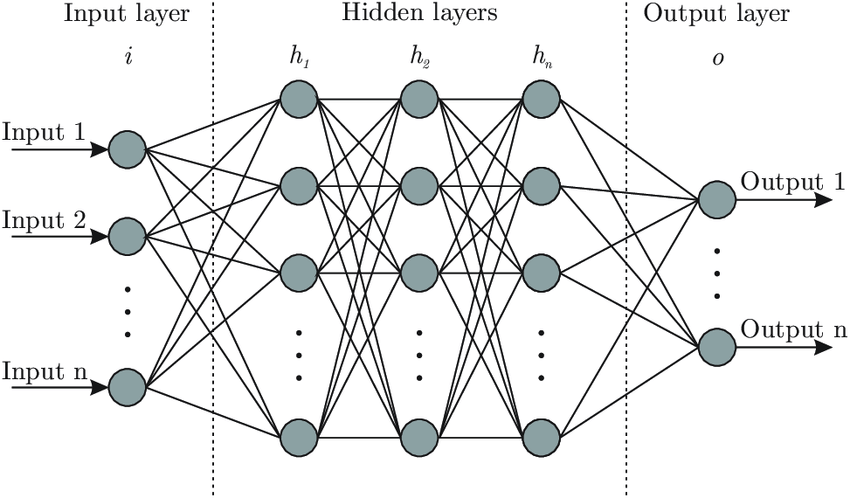
\includegraphics[scale=0.4]{imagens/arch-rede-neural-artificial.png}
    \caption {Arquitetura de uma Rede Neural Artificial \cite{RedeNeuralImagem}.}
\end{figure*}

Elas são compostas por um conjunto interconectado de neurônios artificiais, ou ``nós'', que são organizados em várias camadas, sendo a de entrada responsável por receber os dados, as intermediárias (também conhecidas como camadas ocultas) responsáveis por processar as informações e a de saída responsável por produzir as saídas finais com os resultados da rede neural.

Cada neurônio artificial possui pesos e um valor de viés, sendo o primeiro representando a importância da conexão entre os neurônios, enquanto o segundo é uma medida flexível que facilita a ativação do neurônio de acordo com as preferências incorporadas. Durante o treinamento, os pesos e vieses são ajustados para otimizar o desempenho da rede. A rede funciona por meio de dois processos principais, a propagação direta (do inglês, \textit{forward propagation}), e a retropropagação do erro (do inglês, \textit{backpropagation}). Na propagação direta, os dados de entrada são alimentados na rede neural, passando pelos neurônios e pelas camadas, e resultando em uma saída. Cada neurônio combina linearmente os valores de entrada ponderados pelos pesos, aplica uma função de ativação e repassa o resultado para os neurônios da próxima camada. O erro é calculado em relação aos valores desejados, e a retropropagação do erro ajusta os pesos e vieses dos neurônios para minimizar o erro. Esse processo é repetido até que os pesos sejam ajustados para produzir resultados desejáveis.

Elas são amplamente utilizadas em áreas como visão computacional e processamento de linguagem natural devido à sua capacidade de aprender a partir dos dados e fornecer soluções complexas para problemas desafiadores, capazes de extrair características relevantes dos dados e realizar tarefas como classificação e reconhecimento de padrões.

\subsection{Aprendizado profundo}

O aprendizado profundo (do inglês, \textit{deep learning}) é uma abordagem que utiliza redes neurais artificiais profundas que utilizam múltiplas camadas de processamento interconectadas para extrair representações complexas dos dados com vários níveis de abstração e reconhecimento de padrões. Essas redes neurais profundas são capazes de aprender de forma hierárquica, com cada camada representando características mais abstratas à medida que se aprofunda na rede \cite{AurelienGeron2019}. Essa abordagem permite que o aprendizado profundo seja capaz de lidar com problemas de maior complexidade e extraia automaticamente características relevantes dos dados.

O aprendizado profundo e as redes neurais tem impulsionado significativamente o avanço em áreas como a visão computacional e o processamento de linguagem natural.

\subsection{Aprendizado por conjuntos}

O aprendizado por conjuntos (do inglês, \textit{ensemble learning}) é uma técnica que combina múltiplos modelos de aprendizado de máquina para melhorar o desempenho e a precisão das previsões \cite{OPITZEnsemble}. Ao invés de depender de um único modelo, o aprendizado por conjuntos aproveita a diversidade e a opinião coletiva dos modelos individuais para tomar decisões mais precisas, pois os erros cometidos por um modelo podem ser compensados por outros mais precisos. 

Uma abordagem comum no \textit{ensemble learning} é o \textbf{voto majoritário}, em que cada modelo do conjunto faz uma previsão para uma determinada instância de dados, conhecida como classe, e a classe mais frequente entre os modelos é escolhida como a previsão final. O voto majoritário é simples e eficaz, especialmente quando os modelos individuais têm uma taxa de acerto significativa. Outras estratégias também podem ser utilizadas, como a combinação de probabilidades ou o uso de pesos para ponderar as previsões dos modelos individuais. Essas abordagens levam em consideração a confiança ou a qualidade dos modelos, o que contribui para um aumento geral na precisão das previsões.

Outra abordagem importante de destacar é o uso dos \textbf{hiperparâmetros}, que são parâmetros configuráveis que afetam o desempenho e o comportamento do modelo, influenciando fatores como a complexidade, a velocidade de treinamento e a capacidade de generalização. No \textit{ensemble learning}, os hiperparâmetros são usados para selecionar os modelos de melhor desempenho para o conjunto por meio da busca em grade, que envolve uma grade de valores de hiperparâmetros onde é feita a pesquisa de todas as combinações possíveis desses valores. A seleção adequada dos hiperparâmetros é fundamental para otimizar o desempenho do \textit{ensemble learning} e obter os melhores resultados, da qual requer ajustes dos valores dos hiperparâmetros e avaliação do desempenho do modelo usando métricas apropriadas. Tais métricas são essenciais para avaliar e mensurar os resultados obtidos, sendo elas a acurácia e a AUROC.

A \textbf{acurácia} é uma métrica que avalia a performance de um modelo de aprendizado de máquina, representando a proporção de previsões corretas em relação ao total de previsões realizadas pelo modelo. É calculada dividindo o número de previsões corretas pelo número total de exemplos no conjunto de dados. No entanto, em casos de desbalanceamento de dados, quando uma classe é mais frequente que as outras, a acurácia por si só não é a métrica mais adequada. Nesses casos, é importante considerar outras métricas que possam fornecer uma visão mais abrangente do desempenho do modelo, como a AUROC.

A \textbf{AUROC} (Área sob a Curva Característica de Operação do Receptor) é uma métrica utilizada principalmente para avaliar o desempenho de modelos de classificação binária, como os utilizados em problemas de detecção de conteúdo ofensivo ou não. A curva ROC (Característica de Operação do Receptor) é construída traçando a taxa de verdadeiros positivos em relação à taxa de falsos positivos para diferentes pontos de corte de classificação. A AUROC é a área sob essa curva, variando de 0 a 1, onde um valor mais próximo de 1 indica um modelo com melhor capacidade de distinguir entre as classes. Em geral, uma AUROC de 0,5 indica um modelo com desempenho aleatório, enquanto valores acima de 0,5 indicam um desempenho melhor do que o aleatório \cite{BradleyAUROC}.

\begin{figure*}[!htbp]
	\centering
	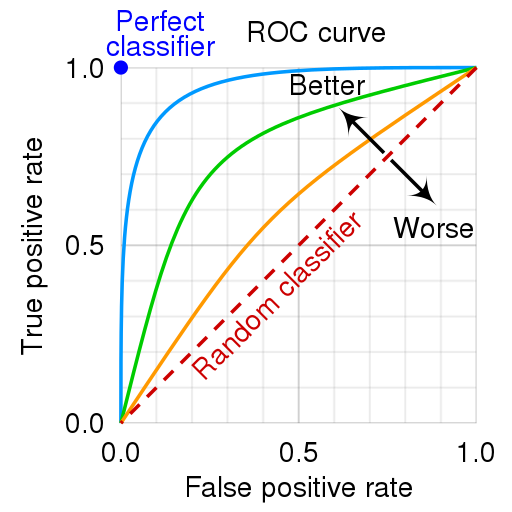
\includegraphics[scale=0.36]{imagens/auroc.png}
    \caption {Curva ROC para um classificador ``melhor'' e ``pior'' \cite{RocCurveWiki}.}
\end{figure*}

O \textit{ensemble learning} é uma técnica amplamente adotada para melhorar a precisão e a estabilidade dos modelos de aprendizado de máquina, frequentemente utilizada em problemas do mundo real, onde a precisão é crucial.

\section{Processamento de Linguagem Natural}

O processamento de linguagem natural (PLN) é uma subárea da inteligência artificial e da linguística que estuda a compreensão e geração automática da linguagem humana. Os sistemas de geração de linguagem natural convertem informação armazenadas em bancos de dados computacionais em linguagem compreensível ao ser humano, enquanto os sistemas de compreensão de linguagem natural convertem ocorrências da linguagem humana em representações mais formais, mais facilmente manipuláveis por programas de computador. O PLN abrange uma variedade de tarefas, como a tradução e geração de respostas automáticas, sumarização de texto, reconhecimento de fala, análise de sentimento, que busca extrair qualidades subjetivas – emoções, humor, sarcasmo, ofensa, motivação, confusão – do texto e muito mais. O objetivo principal do PLN é permitir que os computadores compreendam, interpretem e gerem texto e fala de forma semelhante a linguagem humana\footnote{\textit{What is Natural Language Processing?} | IBM. Disponível em: \url{https://www.ibm.com/topics/natural-language-processing}. Acesso em: 12 de jun. de 2023.}.

Atualmente, os modelos de aprendizagem profunda e as técnicas baseadas em redes neurais possibilitam sistemas de PLN serem capazes de aprender e extrair significados cada vez mais precisos de grandes quantidades de texto bruto. Esses sistemas têm a capacidade de aprimorar seu desempenho à medida que trabalham, permitindo uma compreensão mais avançada da linguagem natural, como os \textit{transformers}.

\subsection{\textit{Transformers}}

Os \textit{transformers} são uma arquitetura de rede neural profunda que revolucionaram o campo do processamento de linguagem natural. Ao contrário das redes neurais convencionais, os \textit{transformers} têm a capacidade de processar informações de uma sequência de entrada de forma simultânea, em vez de depender de um processamento sequencial. Isso permite uma maior paralelização, uma melhor compreensão do contexto global do texto e, consequentemente, uma redução do tempo de treinamento, o que resulta em uma melhoria significativa na eficiência em comparação com as redes neurais tradicionais \cite{GoogleTeamTransformers}. Isso é possível graças ao mecanismo de atenção, que permite que cada elemento da sequência interaja com todos os outros, fornecendo contexto relevante. Os \textit{transformers} têm sido amplamente adotados e são considerados o estado da arte\footnote{\textit{state-of-the-art}. Disponível em: \url{https://www.oxfordlearnersdictionaries.com/definition/english/state-of-the-art}. Acesso em: 12 de jun. de 2023.} no processamento de linguagem natural. Essa designação se refere à abordagem mais avançada e eficaz atualmente disponível no campo do processamento de linguagem natural, baseada em resultados de pesquisa, no desempenho superior em comparação com outras abordagens e na validação em estudos científicos e aplicações práticas.

A arquitetura dos \textit{transformers} é composta por um codificador e um decodificador, ambos contendo várias camadas. O \textbf{codificador} recebe uma sequência de entrada e gera uma representação contextualizada dessa sequência, é responsável por capturar as informações relevantes e as relações entre as palavras ou elementos da sequência. Por sua vez, o \textbf{decodificador} utiliza a representação contextual gerada pelo codificador juntamente com uma sequência de referência para gerar uma sequência de saída, é responsável por produzir a saída desejada com base no contexto e nas informações disponíveis. Ambos utilizam os mecanismos de atenção, autoatenção (do inglês, \textit{self-attention}), atenção de múltiplas cabeças (do inglês \textit{multi-head attention}) e a rede \textit{feed-foward}.

A ``atenção'' é um mecanismo fundamental no processamento de sequências, ela permite que um modelo se concentre em partes relevantes de uma sequência ao ponderar a importância de cada elemento em relação aos outros, calculando sua importância em relação a todos os outros elementos, resultando em uma matriz de pesos de atenção. Já a \textbf{autoatenção} em vez de comparar cada elemento com todos os outros, ela calcula as interações entre os elementos dentro da mesma sequência. Isso é feito por meio de transformações lineares e funções de similaridade, como o a função \textit{softmax}. A autoatenção permite que cada elemento da sequência se relacione com todos os outros elementos, capturando informações contextuais e de dependência importantes. 

Por sua vez, a atenção de múltiplas cabeças permite que o modelo capture informações contextuais de diferentes perspectivas, dividindo a representação de entrada em várias ``cabeças'', cada uma responsável por calcular pesos de atenção que indicam a importância relativa das palavras em relação umas às outras. Os valores são então combinados de acordo com os pesos de atenção, resultando em uma representação ponderada das palavras, que captura relações complexas e melhora a capacidade de representação e aprendizado dos \textit{transformers}.

Por fim, a rede \textit{feed-forward} é um tipo de rede neural, composta por duas camadas lineares com uma função de ativação não linear aplicada entre elas, que é executada individualmente a cada posição na sequência de entrada de forma idêntica. Seu objetivo é fornecer uma transformação não linear que captura padrões complexos e dependências entre os elementos da sequência. Ao introduzir a não linearidade e aprender padrões não lineares, a rede \textit{feed-forward} possibilita que o \textit{transformer} capte informações contextuais e complexas em cada posição da sequência. Isso contribui para a capacidade do modelo de processar efetivamente o contexto da linguagem natural e melhorar o desempenho.

\begin{figure*}[!htbp]
	\centering
	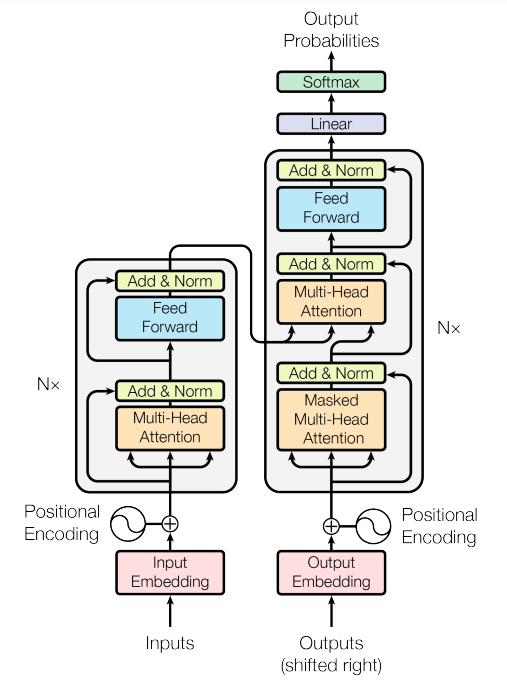
\includegraphics[scale=0.6]{imagens/arch-transformers.png}
    \caption {Modelo de arquitetura de um \textit{transformer} \cite{GoogleTeamTransformers}.}
\end{figure*}

Os \textit{transformers} têm sido amplamente adotados em várias aplicações de PLN e até mesmo em outros domínios, devido à sua capacidade de lidar com sequências de texto de comprimento variável, aprender representações contextualizadas e gerar previsões precisas. Comparados aos modelos de redes neurais, os transformadores são mais receptivos à paralelização, permitindo o treinamento em conjuntos de dados maiores. Isso levou ao desenvolvimento de sistemas pré-treinados, como o BERT e o GPT, que foram treinados com grandes conjuntos de dados de linguagem. Além disso, os \textit{transformers} têm mostrado sucesso não apenas no processamento de linguagem natural, mas também em outras áreas, como visão computacional.

\subsection{BERT}

O BERT (do inglês, \textit{Bidirectional Encoder Representations from Transformers}) é um modelo de linguagem pré-treinado desenvolvido pela \citeonline{BERTImagem}, baseado na arquitetura do \textit{transformer}. Foi treinado em uma grande quantidade de dados não rotulados para aprender representações ricas e contextuais das palavras. O treinamento do BERT envolve duas tarefas principais: ``previsão de máscara'' e ``próxima sentença''. Na previsão de máscara, palavras em uma sequência de texto são mascaradas e o modelo é treinado para prever as palavras mascaradas com base no contexto. Na tarefa de próxima sentença, o BERT aprende a prever se duas sentenças são sequenciais ou não.

O BERT alcançou resultados significativos em várias tarefas de processamento de linguagem natural quando combinado com tarefas de ajuste fino em conjuntos de dados específicos. Ao pré-treinar o modelo em grandes quantidades de dados e depois ajustá-lo para tarefas específicas, o BERT é capaz de capturar nuances semânticas e sintáticas das palavras, melhorando o desempenho em classificação de texto, resposta a perguntas, sumarização e muito mais.

\begin{figure*}[!htbp]
	\centering
	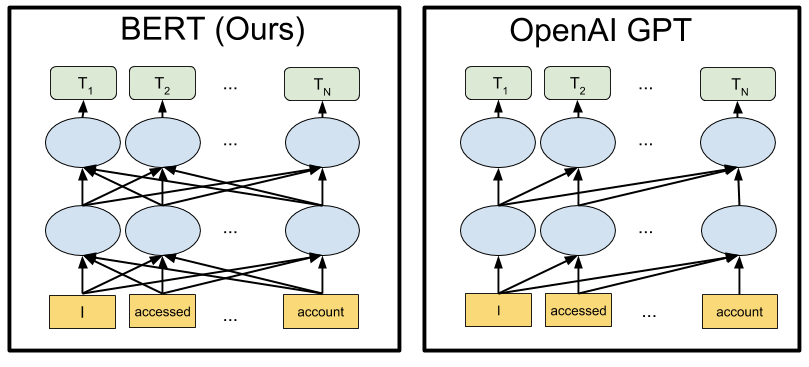
\includegraphics[scale=0.4]{imagens/BERT.png}
    \caption {Representação do BERT (bidirecional), e da OpenAI GPT (unidirecional) \cite{BERTImagem}.}
\end{figure*}

O diferencial do BERT em relação a outros modelos de linguagem pré-treinados é a sua capacidade bidirecional de compreender o contexto das palavras, considerando o contexto anterior e posterior de cada palavra ao realizar o seu processamento, o que permite ao modelo uma melhor compreensão do significado das palavras e frases em um texto, levando em conta as dependências entre elas. Os resultados mostram que modelos de linguagem treinados de forma bidirecional, como o BERT, fornecem uma compreensão mais profunda do contexto linguístico do que os modelos unidirecionais.

\section{Visão Computacional}

A visão computacional é uma área de estudo e aplicação da inteligência artificial que busca capacitar os computadores a interpretarem, analisarem e compreenderem o conteúdo visual de imagens ou vídeos de maneira similar ao ser humano. Isso envolve o desenvolvimento de algoritmos e técnicas que permitem que os sistemas computacionais obtenham informações úteis a partir de dados visuais, e realizem tarefas como reconhecimento facial e de objetos, detecção de padrões, análise de expressões faciais, classificação automática de imagens em redes sociais entre outros\footnote{\textit{What is Computer Vision?} | IBM. Disponível em: \url{https://www.ibm.com/topics/computer-vision}. Acesso em: 12 jun. 2023.}.

A integração de técnicas de visão computacional com outros campos, como processamento de linguagem natural, tem impulsionado pesquisas e avanços significativos na análise e compreensão de dados visuais. Essa integração tem permitido a aplicação de técnicas avançadas de processamento de linguagem natural no campo da visão computacional, resultando em melhorias nas tarefas relacionadas à interpretação e compreensão de informações visuais, como o \textit{VisualBERT}.

\subsection{\textit{VisualBERT}}

O \textit{VisualBERT} é um modelo de linguagem pré-treinado que combina processamento de linguagem natural e a visão computacional para entender e interpretar informações visuais e textuais simultaneamente, baseado na arquitetura do BERT, ao contrário dos modelos que se baseiam apenas em texto, ele incorpora também representações visuais das imagens para melhorar o desempenho em tarefas que envolvem texto e contexto visual. O modelo é treinado em um grande conjunto de dados multimodais que combina texto descritivo e imagens correspondentes, tal abordagem permite que o \textit{VisualBERT} capture informações visuais relevantes, permitindo uma melhor compreensão de textos relacionados a imagens e aprimorando o desempenho em tarefas como descrição de imagens, geração de legendas entre outros. O \textit{VisualBERT} representa uma extensão dos modelos de linguagem pré-treinados, integrando efetivamente a visão computacional ao processamento de linguagem natural para uma análise mais completa e precisa de conteúdos multimodais \cite{VisualBERTArt}.

O \textit{VisualBERT} é pré-treinado usando dois objetivos semelhantes aos usados no BERT: modelagem de linguagem mascarada com previsão de alinhamento de imagens e legendas. O processo de pré-treinamento envolve treinar o modelo com um grande conjunto de dados multimodais que combinam texto descritivo e imagens correspondentes, para prever alguma parte oculta (mascarada) da entrada, seja uma parte de uma imagem ou uma palavra do texto. Após o pré-treinamento, o modelo passa por um processo de ajuste fino em conjuntos de dados específicos para aprimorar seu desempenho. Isso permite que o modelo se adapte às características e nuances das tarefas específicas, refinando ainda mais suas representações multimodais.

A arquitetura do \textit{VisualBERT} utiliza uma camada de entrada compartilhada para codificar tanto o texto quanto as representações visuais. Utilizando técnicas de codificação de palavras e redes neurais, essa camada captura informações contextuais das palavras e das representações visuais por meio de várias camadas do codificador do \textit{transformer}, assim como o BERT. Cada camada do codificador possui subcamadas de atenção \textit{multi-head} e redes \textit{feed-forward}, permitindo a captura de interações e padrões entre palavras e informações visuais. Os recursos visuais extraídos das propostas de objetos são tratados como \textit{tokens} de entrada não ordenados e incorporados no \textit{VisualBERT} juntamente com o texto. Essa abordagem permite que o modelo capture e relacione informações tanto textuais quanto visuais, permitindo uma compreensão mais completa dos dados multimodais.

\begin{figure*}[!htbp]
	\centering
	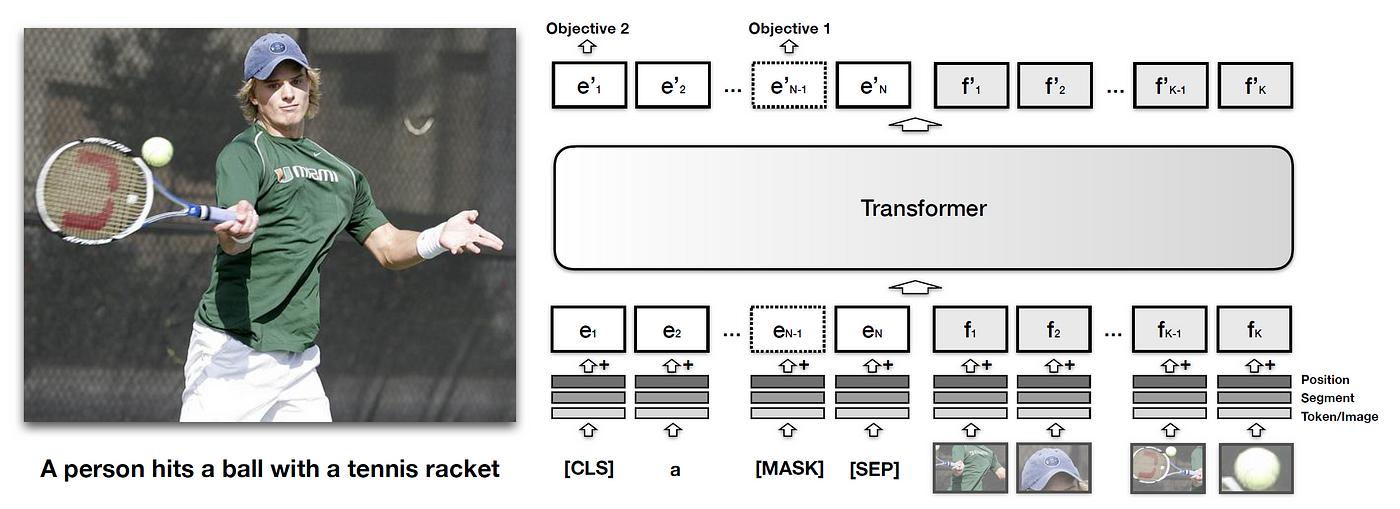
\includegraphics[scale=0.35]{imagens/visualBERT.png}
    \caption {Arquitetura do \textit{VisualBERT} \cite{VisualBERTArt}.}
\end{figure*}

\section{Multimodalidade}

A multimodalidade refere-se à capacidade de combinar e integrar múltiplas modalidades de comunicação, como texto, imagem, som, gestos e outros elementos sensoriais, para transmitir ou compreender informações de maneira mais rica e completa\footnote{\textit{What is Multimodal?} | \textit{University of Illinois Springfield}. Disponível em: \url{https://www.uis.edu/learning-hub/writing-resources/handouts/learning-hub/what-is-multimodal}. Acesso em: 12 jun. 2023.}. É a interação entre diferentes formas de representação e expressão que enriquece a comunicação e permite uma compreensão mais abrangente do conteúdo, permitindo uma comunicação mais rica e eficaz entre humanos e máquinas.

Ao lidar com a multimodalidade, os sistemas computacionais buscam interpretar e extrair informações de diferentes modalidades, permitindo que os usuários se envolvam de maneira mais natural e efetiva com a tecnologia. Essa abordagem é amplamente aplicada em áreas como processamento de linguagem natural, visão computacional, interação humano-computador e aprendizado de máquina, onde a combinação de modalidades permite uma compreensão mais rica e abrangente dos dados. Ao combinar informações de várias modalidades, é possível melhorar o desempenho de uma variedade de tarefas, resultando em soluções mais eficazes para uma ampla gama de desafios.

\section{Trabalhos Relacionados}

\subsection{Desafio dos Memes Odiosos (\textit{The Hateful Memes Challenge})} 

Este trabalho realizado pela equipe da Meta AI \cite{ArticleHatefulMemesChallenge2021} propôs um desafio para a classificação multimodal, com foco na detecção de discurso de ódio em memes multimodais. Fornecem modelos multimodais com diferentes níveis de sofisticação e ilustram como foi feita a criação do banco de dados com os memes odiosos e os memes categorizados como “confundidores benignos”. Esses confundidores foram adicionados ao conjunto de dados para aumentar a dificuldade do desafio, pois usam as mesmas imagens e frases que os memes odiosos, mas em contextos que não se enquadram como discurso de ódio. O objetivo deste desafio foi estimular a inovação e impulsionar o progresso no raciocínio e compreensão multimodal, que podem ter impactos positivos em várias tarefas e aplicações, ao mesmo tempo em que facilita o progresso da detecção de discurso de ódio e seu combate por meio de métodos automáticos.

\subsection{Detectando Discurso de Ódio em Memes Usando Abordagens de Aprendizado Profundo Multimodal} 

Os participantes do desafio proposto pela Meta IA adotaram uma abordagem que consistiu, primeiramente, em expandir o conjunto de treinamento por meio da busca por conjuntos de dados semelhantes na web. Em seguida, foram extraídas características das imagens utilizando algoritmos de detecção de objetos (\textit{Detectron}), o que permitiu aprimorar o modelo pré-treinado (\textit{VisualBERT}). Por fim, foi realizada a pesquisa de hiperparâmetros e aplicada a técnica de voto majoritário, atingindo 0,811 AUROC com uma precisão de 0,765 no conjunto de teste do desafio \cite{velioglu2020hateful}.
% Vision Models Are More Robust And Fair When Pretrained On Uncurated Images Without Supervision: https://arxiv.org/pdf/2202.08360v2.pdf

% Metodologia: Explicação detalhada do método de pesquisa utilizado (quantitativa, qualitativa, estudo de caso, revisão sistemática etc.).

% Contextualização: Apresentação do contexto ou cenário relacionado ao tema (histórico, cultural, social, econômico, entre outros).

% Treinamento, Classificação

% Análise de Dados/Resultados: Apresentação, descrição e interpretação dos dados coletados ou das análises realizadas.

% Discussão: Comparação dos resultados com a literatura existente, reflexões e implicações teóricas ou práticas.

% Limitações da Pesquisa: Identificação de possíveis limitações no estudo, como escopo, recursos ou tempo.

% O Google Colab é um serviço do Jupyter Notebook hospedado que oferece acesso gratuito a recursos de computação, incluindo GPUs e TPUs. Ele é adequado principalmente para aprendizado de máquina, ciência de dados e educação. 

\chapter{Desenvolvimento}
\label{cap:03}

\section{MMF}

O MMF, é um framework modular para pesquisa de visão e linguagem multimodal de código aberto criado pelo Facebook AI Research (FAIR). É considerado o estado da arte (state-of-the-art) desse seguimento, onde foi utilizado como referência para desenvolver projetos como o Visualbert.

Já o Detectron2 é uma plataforma também de código aberto para detecção de objetos, segmentação e outras tarefas de reconhecimento visual. Também é considerado o estado da arte em detecção e segmentação, onde oferece suporte a vários projetos de pesquisa de visão computacional.

PyTorch é uma biblioteca de aprendizado de máquina em código aberto usada para implementações de aprendizado profundo, como visão computacional (usando TorchVision) e processamento de linguagem natural

\begin{figure*}[!htbp]
	\centering
	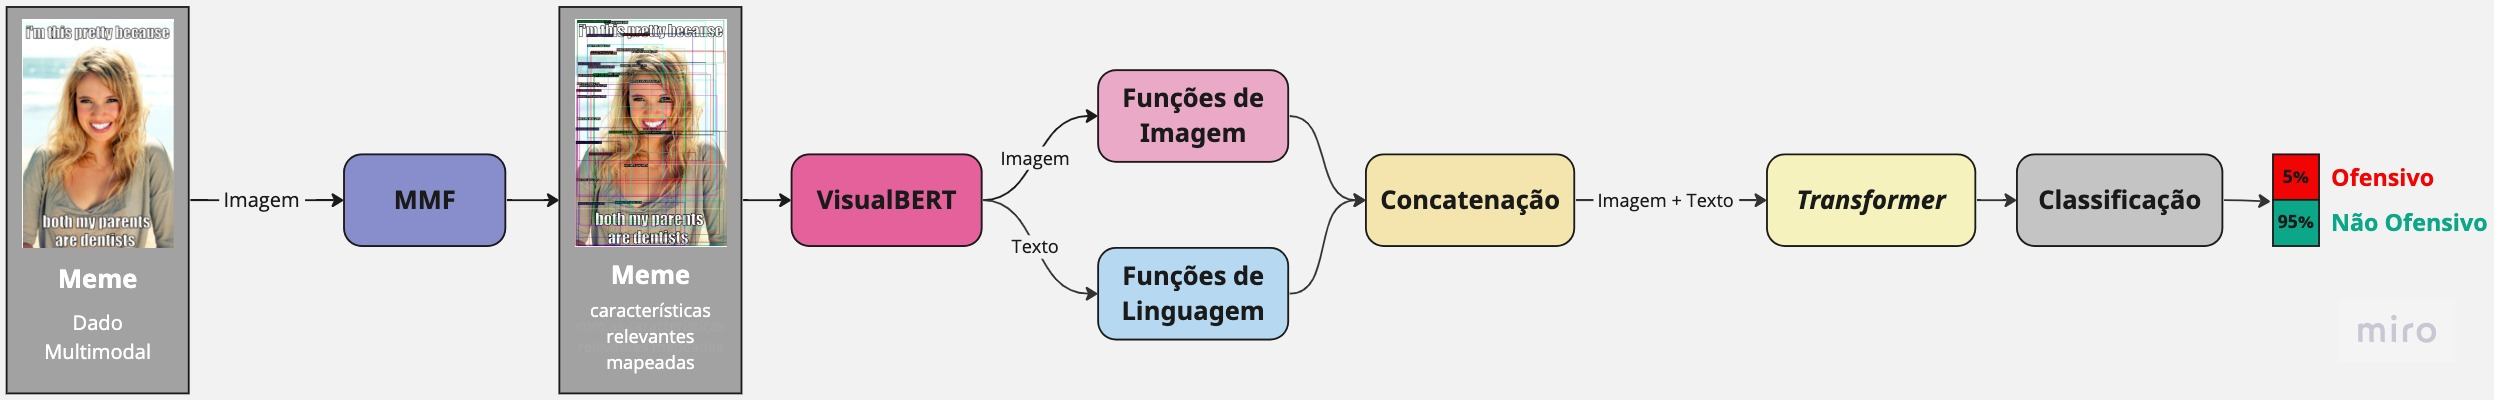
\includegraphics[scale=0.18]{imagens/diagrama.jpeg}
    \caption {Arquitetura da Proposta de Desenvolvimento.}
\end{figure*}


% \section{Proposta}

% Para iniciar o projeto, será utilizado o banco de dados de memes odiosos criado pela Meta, composto por 10 mil memes em inglês que contêm conteúdo ofensivo relacionado a gênero, raça, religião, orientação sexual, classe social e outros tópicos. Dada à sensibilidade desses dados, eles só estão disponíveis para pesquisas que estejam em conformidade com os termos de uso referentes a sua utilização, compartilhamento e armazenamento. O conjunto de dados é composto pelas seguintes porcentagens: 40\% de memes de ódio multimodal, 10\% de memes de ódio unimodal, 20\% de memes com confusão de texto benigna, 20\% de memes com confusão de imagem benigna e 10\% de memes não odiosos aleatórios. Os ``confundidores benignos'' consistem em imagens ou textos alternativos para cada meme odioso, que alteram sua classificação para não odioso. Esses confundidores foram adicionados para garantir que o conjunto de dados seja apropriado para testar a verdadeira capacidade multimodal de um modelo, levando em conta que, no mundo real, o modelo se depararia com exemplos diversos e inéditos.

% Dando sequência no desenvolvimento do trabalho, será utilizado o modelo MMF, uma estrutura pré-definida com funcionalidades para pesquisa multimodal de visão e linguagem fornecida pelo \textit{Facebook AI Research}\footnote{MMF: \textit{a framework for vision-and-language multimodal research from Facebook AI Research} (FAIR). 2020. Disponível em: \url{https://github.com/facebookresearch/mmf}. Acesso em: 24 de mai. de 2023.}. Esse modelo será aplicado para detectar objetos e extrair características relevantes das imagens presentes no banco de dados, seu funcionamento consiste em receber uma imagem de entrada e produzir uma coleção de caixas delimitadoras, cada uma contendo um objeto identificado, juntamente com sua categoria, como por exemplo, animal ou humano. Essa abordagem visa aprimorar o desempenho do \textit{VisualBERT}, um modelo já pré-treinado com um vasto conjunto de dados de legenda e imagem.

% O conjunto de dados de memes odiosos não tem o propósito de treinar o modelo do \textit{VisualBERT} a partir do zero, mas sim de ajustá-lo e testá-lo, a fim de reduzir o viés e possibilitar uma identificação e classificação mais eficiente de memes considerados como odiosos ou ofensivos. Para atingir esse objetivo, será utilizado o método de aprendizagem supervisionada, combinado com o aprendizado profundo e por conjuntos, utilizando a métrica primária de área sob a curva característica de operação do receptor (AUROC) e a acurácia para avaliar a eficiência e a precisão do modelo, o objetivo é alcançar métricas com um valor igual ou superior a 0,7.


% % A AUROC é uma medida que avalia a capacidade do modelo em distinguir corretamente as classes positiva e negativa, enquanto a acurácia mede a proporção de predições corretas em relação ao total de predições. Essas métricas serão fundamentais para garantir a qualidade e confiabilidade dos resultados obtidos pelo modelo.

% A etapa de treinamento e aprendizado onde serão os maiores desafios do projeto, pois requer ajustes finos usando a rede neural aprendida como base para obter melhores resultados no processo de reconhecimento de padrões. A cada certa atualização do modelo é realizada uma nova avaliação no conjunto de validação, utilizando uma taxa de aprendizado definida para controlar as etapas de atualização de treinamento durante o ajuste fino. Uma pesquisa de hiperparâmetros é conduzida para encontrar a configuração ideal, na qual o modelo é avaliado com diferentes conjuntos de hiperparâmetros, considerando suas pontuações de AUROC. Por fim, a técnica de votação majoritária é aplicada para realizar a classificação binária final dos memes multimodais, distinguindo entre os ofensivos e não ofensivos. 

% % O ajuste fino é uma técnica comum em aprendizado profundo que envolve a adaptação de um modelo pré-treinado a uma tarefa downstream específica, treinando-o em dados específicos da tarefa. O modelo VisualBERT ajustado é então usado para fazer previsões sobre novos memes. Além disso, o projeto usa aprendizado conjunto, que é uma técnica que combina as previsões de vários modelos para melhorar o desempenho. A abordagem de conjunto usa vários modelos de aprendizado profundo que são ajustados em diferentes subconjuntos dos dados de treinamento para melhorar o desempenho geral do sistema.

% % Por fim, a abordagem aplica aprendizado conjunto para combinar as previsões de vários modelos para melhorar o desempenho. A abordagem alcançou um AUROC de 0,811 e uma precisão de 0,765 no conjunto de teste de desafio

% % Fazer pré-treinamento em grandes conjuntos de dados reduz a variância, mas aumenta o viés. Além disso, aumentar o tamanho do conjunto de dados nem sempre melhora o desempenho. Por exemplo, [80] observaram que o tamanho do conjunto de dados não é o fator mais importante no pré-treinamento visual-linguístico. Eles afirmam que mesmo um conjunto de dados menor pode facilmente superar o pré-treinamento em um conjunto de dados maior quando o domínio visual e textual correto corresponde a dados de boa qualidade.

% % Realizamos uma extensa pesquisa de hiperparâmetros e usamos a melhor configuração para os parâmetros, incluindo taxa de aprendizado, etapas de aquecimento, tipo de aquecimento, fator de aquecimento e iterações de aquecimento. Avaliamos os modelos com diferentes hiperparâmetros durante a busca da grade e os 27 melhores modelos, de acordo com suas pontuações AUROC, são conjuntos. Finalmente, a técnica de votação por maioria é aplicada para finalizar a classificação.

% \section{Cronograma}

% Como forma de organizar e alcançar os objetivos deste trabalho no próximo semestre, será adotada a metodologia SCRUM, um \textit{framework} ágil utilizado no gerenciamento de projetos, especialmente no desenvolvimento de \textit{software} \cite{MicheleSligerSCRUM}. É conhecido por promover a flexibilidade e adaptabilidade, permitindo uma resposta ágil a mudanças e prioridades. E com base nessa metodologia, o trabalho será organizado adaptando os ciclos característicos do SCRUM para melhor atender às necessidades do projeto.

% \begin{figure*}[!htbp]
% 	\centering
% 	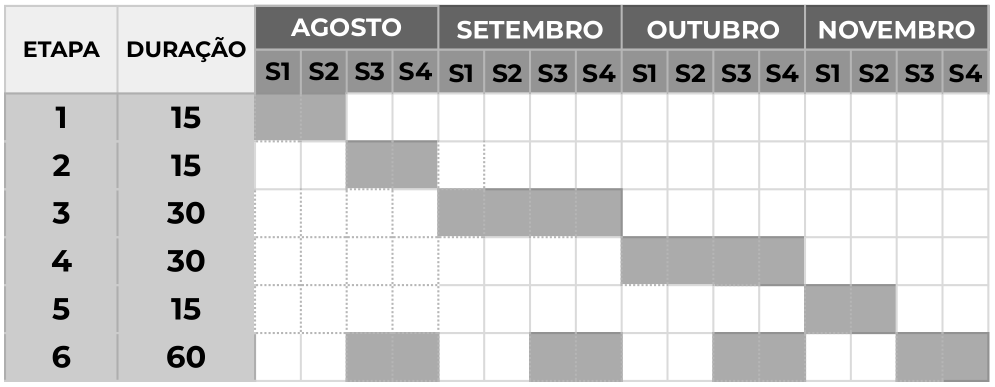
\includegraphics[scale=0.9]{imagens/cronograma}
%     \caption {Cronograma proposto: \textbf{Etapa 1.} Extração de características relevantes das imagens do banco de dados; \textbf{Etapa 2.} Utilização do modelo do \textit{VisualBERT}; \textbf{Etapa 3.} Treinamento; \textbf{Etapa 4.} Classificação dos memes; \textbf{Etapa 5.} Testes, análises e levantamento dos resultados; \textbf{Etapa 6.} Documentação.}
% \end{figure*}

% O trabalho será dividido em seis etapas, em que cada uma delas terá uma lista de tarefas que incluirão funcionalidades, requisitos e melhorias a serem implementadas. Para organizar o desenvolvimento do projeto, serão adotados ciclos chamados \textit{sprints}, com duração de 2 semanas. No início de cada \textit{sprint}, um conjunto de tarefas será selecionado para desenvolvimento dentro do prazo estabelecido, utilizando o método \textit{Kanban}, onde as tarefas serão divididas em colunas representando as etapas de ``a fazer'', ``em desenvolvimento'' e ``concluídas''. E ao final de cada \textit{sprint}, planejo fazer uma revisão do trabalho realizado para identificar pontos de melhoria e ajustes para os próximos \textit{sprints}. Esses pontos poderão ser compartilhados e discutidos em conjunto com o orientador do trabalho.

% Detalhando melhor as etapas do cronograma, a primeira \textit{sprint} irá começar com a utilização do \textit{framework} MMF para extrair características relevantes das imagens do banco de dados de memes odiosos, juntamente com o preparo do ambiente de desenvolvimento. Após a utilização e familiaridade com a ferramenta, a próxima \textit{sprint} será dedicada à utilização do modelo \textit{VisualBERT} com as imagens já tratadas pelo MMF. Em seguida, serão necessárias duas sprints para realizar o treinamento, em seguida mais duas \textit{sprints} para a classificação dos memes com base nesse treinamento. Após a conclusão dessas etapas, será realizada uma \textit{sprint} de testes e análises dos resultados obtidos, e caso necessário, haverá a possibilidade de retornar às etapas de treinamento e classificação para realizar melhorias adicionais. Além disso, será feito um levantamento de todos os resultados interessantes, que serão apresentados e detalhados. Por fim, a cada uma \textit{sprint}, a documentação será atualizada com o passo a passo detalhado de como as etapas foram realizadas, garantindo um registro claro e organizado do progresso e das decisões tomadas ao longo do projeto.
%\input{cap4resultados}
%\input{cap5conclusao}

% ----------------------------------------------------------
% ELEMENTOS PÓS-TEXTUAIS
% ----------------------------------------------------------
\postextual
% ----------------------------------------------------------

% ----------------------------------------------------------
% Referências bibliográficas
% ----------------------------------------------------------
\bibliography{referencias}

% ----------------------------------------------------------
% Glossário
% ----------------------------------------------------------
%
% Consulte o manual da classe abntex2 para orientações sobre o glossário.
%
%\glossary

% ----------------------------------------------------------
% Apêndices
% ----------------------------------------------------------

% ---
% Inicia os apêndices
% ---
%% Texto ou documento elaborado pelo autor, a fim de complementar sua argumentação, sem prejuízo da unidade nuclear do trabalho.

% ---
% Inicia os apêndices
% ---
\begin{apendicesenv}
	
	% Imprime uma página indicando o início dos apêndices
	\partapendices
	
	% ----------------------------------------------------------
	\chapter{Título do Apêndice A}
	% ----------------------------------------------------------
	
	Texto do Apêndice A.
	
	
	
	% ----------------------------------------------------------
	\chapter{Título do Apêndice B}
	% ----------------------------------------------------------
	
	Texto do Apêndice B.
	
	
	
	
\end{apendicesenv}
% ---
% ---


% ----------------------------------------------------------
% Anexos
% ----------------------------------------------------------

% ---
% Inicia os anexos
% ---
%\begin{anexosenv}

% Imprime uma página indicando o início dos anexos
\partanexos

% ---
\chapter{Morbi ultrices rutrum lorem.}
% ---
\lipsum[30]

\end{anexosenv}

%---------------------------------------------------------------------
% INDICE REMISSIVO
%---------------------------------------------------------------------
%\phantompart
\printindex
%---------------------------------------------------------------------

\end{document}
